\pdfminorversion=3
\documentclass[tikz,border={0mm 8mm 2mm 0mm}]{standalone}
\usepackage{vuiprepstandalone}
\usepackage{alain2}
\usepackage{pifont}
%\newcommand{\cmark}{\ding{51}}%
%\newcommand{\xmark}{\ding{55}}%
\def\pathfig{CHAP3/ex_Shell/images/}
\usetikzlibrary{decorations,calc}
\usepackage[locale=FR]{siunitx}

\begin{document}

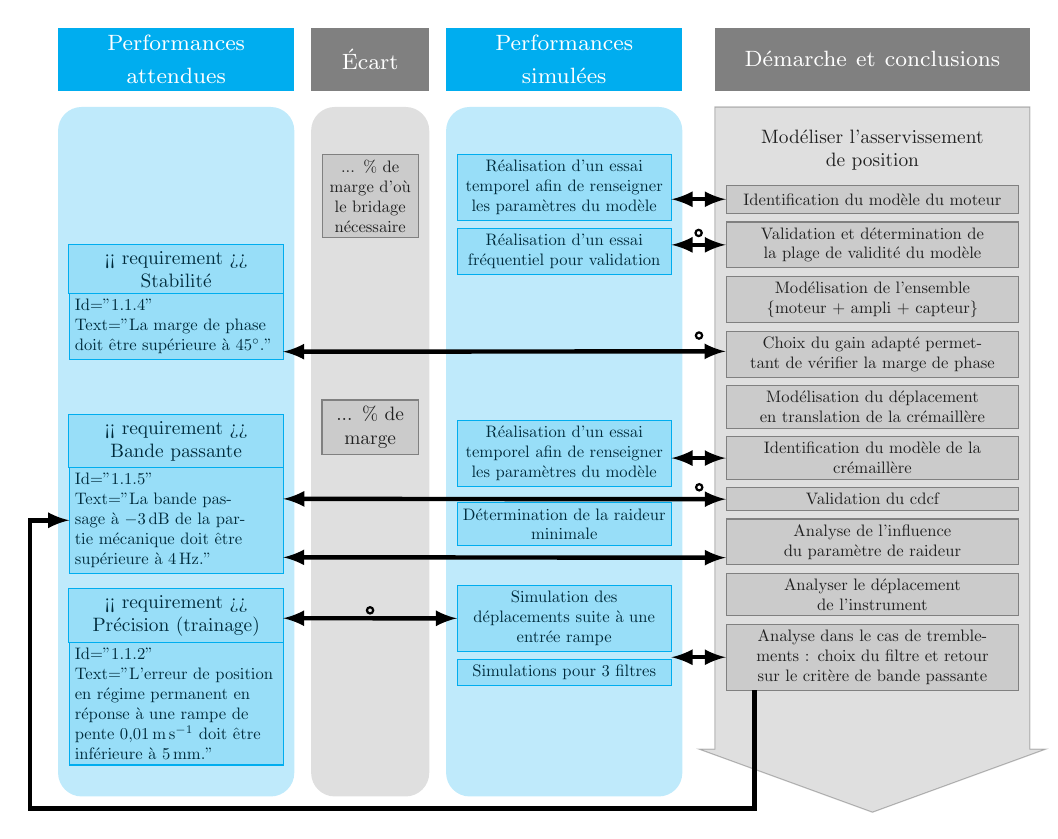
\begin{tikzpicture}

\begin{scope}
\node[white,fill=cyan,align=center,text width=3cm-4pt,inner sep=2pt,minimum height=.8cm] (a) {\footnotesize Performances\\ attendues}; 
%%% A COMPLETER AVEC LES NOEUDS VOULUS
\node[anchor=north,draw=cyan,fill=cyan!20,rectangle,outer sep=0pt,align=center,text width={(2.5cm+1em/3)/.7-1em/3*.7},scale=.7] (adebut) at ($(a.south)+(0,-1.95)$)  {<< requirement >> \\  Stabilité};
\node[anchor=north,draw=cyan,fill=cyan!20,rectangle,outer sep=0pt,align=left,text width={(2.5cm+1em/3)/.6-1em/3*.6},align=left,scale=.6] (adebut2) at (adebut.south)  {Id="1.1.4"\\ Text="La marge de phase doit être supérieure à \SI{45}{\degree}."};


\node[anchor=north,draw=cyan,fill=cyan!20,rectangle,outer sep=0pt,align=center,text width={(2.5cm+1em/3)/.7-1em/3*.7},scale=.7] (a11) at ($(adebut2.south)+(0,-.7)$)   {<< requirement >> \\ Bande passante};
\node[anchor=north,draw=cyan,fill=cyan!20,rectangle,outer sep=0pt,text width={(2.5cm+1em/3)/.6-1em/3*.6},align=left,scale=.6] (a12) at (a11.south)  {Id="1.1.5"\\ Text="La bande passage à \SI{-3}{dB} de la partie mécanique doit être supérieure à \SI{4}{Hz}."};

\node[anchor=north,draw=cyan,fill=cyan!20,rectangle,outer sep=0pt,align=center,text width={(2.5cm+1em/3)/.7-1em/3*.7},scale=.7] (afin0) at ($(a12.south)+(0,-.2)$)   {<< requirement >> \\ Précision (trainage)};
\node[anchor=north,draw=cyan,fill=cyan!20,rectangle,outer sep=0pt,text width={(2.5cm+1em/3)/.6-1em/3*.6},align=left,scale=.6] (afin) at (afin0.south)  {Id="1.1.2"\\ Text="L'erreur de position en régime permanent en réponse à une rampe de pente \SI{0.01}{m.s^{-1}} doit être inférieure à \SI{5}{mm}."};

\end{scope}

\begin{scope}
\node[white,fill=gray,align=center,text width=1.5cm-4pt,inner sep=2pt,minimum height=.8cm,anchor=west,xshift=.2cm]  (b) at (a.east) {\footnotesize \'Ecart}; 
%%% A COMPLETER AVEC LES NOEUDS VOULUS
\node[text width={(1cm+1em/3)/.6-1em/3*.6},scale=.6,anchor=north,,draw=gray,fill=gray!20,align=center,rectangle] (bdebut) at ($(b.south)+(0,-.8)$)   {... \% de marge d'où le bridage nécessaire};
\node[text width={(1cm+1em/3)/.7-1em/3*.7},scale=.7,anchor=north,,draw=gray,fill=gray!20,align=center,rectangle] (bfin) at ($(bdebut.south)+(0,-2.05)$)   {... \% de marge  };
\end{scope}

\begin{scope}
\node[white,fill=cyan,align=center,text width=3cm-4pt,inner sep=2pt,minimum height=.8cm,anchor=west,xshift=.2cm]  (c) at (b.east) {\footnotesize Performances \\ simulées}; 
%%% A COMPLETER AVEC LES NOEUDS VOULUS
\node[text width={(2.5cm+1em/3)/.6-1em/3*.6},scale=.6,anchor=north,draw=cyan,fill=cyan!20,rectangle,text badly centered] (cdebut) at ($(c.south)+(0,-.8)$)   {Réalisation d'un essai temporel afin de renseigner les paramètres du modèle};
\node[text width={(2.5cm+1em/3)/.6-1em/3*.6},scale=.6,anchor=north,draw=cyan,fill=cyan!20,rectangle,text badly centered] (c2) at ($(cdebut.south)+(0,-.1)$)   {Réalisation d'un essai fréquentiel pour validation};
\node[text width={(2.5cm+1em/3)/.6-1em/3*.6},scale=.6,anchor=north,draw=cyan,fill=cyan!20,rectangle,text badly centered] (c3) at ($(c2.south)+(0,-1.85)$)   {Réalisation d'un essai temporel afin de renseigner les paramètres du modèle};
\node[text width={(2.5cm+1em/3)/.6-1em/3*.6},scale=.6,anchor=north,draw=cyan,fill=cyan!20,rectangle,text badly centered] (c4) at ($(c3.south)+(0,-.2)$)   {Détermination de la raideur minimale};
\node[text width={(2.5cm+1em/3)/.6-1em/3*.6},scale=.6,anchor=north,draw=cyan,fill=cyan!20,rectangle,text badly centered] (c5) at ($(c4.south)+(0,-.5)$)   {Simulation des déplacements suite à une entrée rampe};
\node[text width={(2.5cm+1em/3)/.6-1em/3*.6},scale=.6,anchor=north,draw=cyan,fill=cyan!20,rectangle,text badly centered] (cfin) at ($(c5.south)+(0,-.1)$)   {Simulations pour 3 filtres};
\end{scope}

\begin{scope}
\node[white,fill=gray,align=center,text width=4cm-4pt,inner sep=2pt,minimum height=.8cm,anchor=west,xshift=.4cm]  (d) at (c.east) {\footnotesize Démarche et conclusions}; 
%%% A COMPLETER AVEC LES NOEUDS VOULUS
\node[text width={(3.5cm+1em/3)/.7-1em/3*.7},scale=.7,anchor=north,minimum height=.6cm, align=center] (ddebut) at ($(d.south)+(0,-.4)$)   {Modéliser l'asservissement de position};
\node[text width={(3.5cm+1em/3)/.6-1em/3*.6},scale=.6,anchor=north,draw=gray,fill=gray!20,rectangle,minimum height=.6cm, align=center] (d2) at ($(ddebut.south)+(0,-.1)$)   {Identification du modèle du moteur};
\node[text width={(3.5cm+1em/3)/.6-1em/3*.6},scale=.6,anchor=north,draw=gray,fill=gray!20,rectangle,minimum height=.6cm, align=center] (d3) at ($(d2.south)+(0,-.1)$)   {Validation et détermination de la plage de validité du modèle};
\node[text width={(3.5cm+1em/3)/.6-1em/3*.6},scale=.6,anchor=north,draw=gray,rectangle,fill=gray!20,align=center,minimum height=0cm] (d4) at ($(d3.south)+(0,-.1)$)   {Modélisation de l'ensemble \{moteur + ampli + capteur\}};
\node[text width={(3.5cm+1em/3)/.6-1em/3*.6},scale=.6,anchor=north,draw=gray,rectangle,fill=gray!20,align=center,minimum height=0cm] (d5) at ($(d4.south)+(0,-.1)$)   {Choix du gain adapté permettant de vérifier la marge de phase};
\node[text width={(3.5cm+1em/3)/.6-1em/3*.6},scale=.6,anchor=north,draw=gray,rectangle,fill=gray!20,align=center,minimum height=0cm] (d6) at ($(d5.south)+(0,-.1)$)   {Modélisation du déplacement en translation de la crémaillère};
\node[text width={(3.5cm+1em/3)/.6-1em/3*.6},scale=.6,anchor=north,draw=gray,rectangle,fill=gray!20,align=center,minimum height=0cm,text badly centered] (d7) at ($(d6.south)+(0,-.1)$)   {Identification du modèle de la crémaillère};
\node[text width={(3.5cm+1em/3)/.6-1em/3*.6},scale=.6,anchor=north,draw=gray,rectangle,fill=gray!20,align=center,minimum height=0cm] (d8) at ($(d7.south)+(0,-.1)$)   {Validation du cdcf};
\node[text width={(3.5cm+1em/3)/.6-1em/3*.6},scale=.6,anchor=north,draw=gray,rectangle,fill=gray!20,align=center,minimum height=0cm] (d9) at ($(d8.south)+(0,-.1)$)   {Analyse de l'influence du paramètre de raideur};
\node[text width={(3.5cm+1em/3)/.6-1em/3*.6},scale=.6,anchor=north,draw=gray,rectangle,fill=gray!20,align=center,minimum height=0cm] (d10) at ($(d9.south)+(0,-.1)$)   {Analyser le déplacement de l'instrument};
\node[text width={(3.5cm+1em/3)/.6-1em/3*.6},scale=.6,anchor=north,draw=gray,rectangle,fill=gray!20,align=center,minimum height=0cm] (dfin) at ($(d10.south)+(0,-.1)$)   {Analyse dans le cas de tremblements : choix du filtre et retour sur le critère de bande passante};
\end{scope}

%%% OVERLAY DE LA FIN
%%%%
\coordinate (ymin) at ($(afin.south)+(0,0.2)$);
\coordinate (ymax) at ($(ddebut.north)$);

\draw[rounded corners = .3cm,draw=none, fill=cyan, opacity=.25, remember picture, overlay] ($(afin.south)!(ymax)!(afin.north)+(-1.5,.2)$) rectangle ($(afin.south)!(ymin)!(afin.north)+(1.5,-.6)$);
\draw[rounded corners = .3cm,draw=none, fill=gray, opacity=.25, remember picture, overlay] ($(bfin.south)!(ymax)!(bfin.north)+(-.75,.2)$) rectangle ($(bfin.south)!(ymin)!(bfin.north)+(.75,-.6)$);
\draw[rounded corners = .3cm,draw=none, fill=cyan, opacity=.25, remember picture, overlay] ($(cfin.south)!(ymax)!(cfin.north)+(-1.5,.2)$) rectangle ($(cfin.south)!(ymin)!(cfin.north)+(1.5,-.6)$);
%\draw[rounded corners = .3cm,draw=none, fill=gray, opacity=.25, remember picture, overlay] ($(ddebut.north)+(-2.,.2)$) rectangle ($(dfin.south)!(ymin)!(dfin.north)+(2.,-.2)$);
\draw[draw=black, fill=gray, opacity=.25, remember picture, overlay] ($(dfin.south)!(ymax)!(dfin.north)+(-2.,.2)$) |- ($(dfin.south)!(ymin)!(dfin.north)+(160:2.341)+(0,-.8)$) -- ++(-20:2.341) -- ++(20:2.341) -| ($(dfin.south)!(ymax)!(dfin.north)+(2.,.2)$) -- cycle;
%%% FLECHE DE FIN
\draw[ultra thick,<->,>=latex] ($(adebut2.south east)+(0,.1)$) -- ($(dfin.west)!($(adebut2.south east)+(0,.1)$)!(ddebut.west)$) node[above,draw, circle,inner sep=1pt,thick,pos=.94,yshift=1.5mm,scale=.8] {\footnotesize\cmark};
\draw[ultra thick,<->,>=latex] ($(d8.west)$) -- ($(afin.east)!(d8.west)!(adebut.east)$) node[above,draw, circle,inner sep=1pt,thick,pos=.06,yshift=1.mm,scale=.8] {\footnotesize\cmark};
\draw[ultra thick,<->,>=latex] ($(d9.west)+(0,-.2)$) -- ($(afin.east)!($(d9.west)+(0,-.2)$)!(adebut.east)$);% node[below,draw, circle,inner sep=1pt,thick,pos=.06,yshift=-1.5mm] {\footnotesize\cmark};
\draw[ultra thick,<->,>=latex] ($(c5.west)+(0,0)$) -- ($(afin.east)!($(c5.west)+(0,0)$)!(adebut.east)$) node[above,draw, circle,inner sep=1pt,thick,midway,yshift=.5mm,scale=.8] {\footnotesize\cmark};


\draw[ultra thick,<->,>=latex]  ($(cdebut.east)!(d2.west)!(c2.east)$) -- (d2.west);
\draw[ultra thick,<->,>=latex]  ($(cdebut.east)!(d3.west)!(c2.east)$) -- (d3.west) node[above,draw, circle,inner sep=1pt,thick,midway,yshift=1mm,scale=.8] {\footnotesize\cmark};;
\draw[ultra thick,<->,>=latex]  ($(cdebut.east)!(d7.west)!(c2.east)$) -- (d7.west);
\draw[ultra thick,<->,>=latex]  ($(cdebut.east)!(dfin.west)!(c2.east)$) -- (dfin.west) ;

\draw[ultra thick,->,>=latex] ($(dfin.south)+(-1.5,0)$) |- ++(-9.2,-1.5) |- (a12.west);
\end{tikzpicture}

\end{document}